\section{Act 3: Visualizing and analyzing ET data with GMEMs and GAMMs}

We observed nearly identical time course of predictive processing, see figure \ref{fig:comparitive}, in which restricted sentences resulted in earlier looks to the target object than nonrestrictive sentences. Both GLMER and GAMMS require specific coding of the data for the model to predict in the expected manner. However, each of these models start with coding the data correctly and building maximal models and working down to simpler models for model comparison. \parencite{max model}. Visualizations for model outputs will be provided.

\subsection{Visualizations}
While 

\lstinputlisting[language=R, firstnumber=last]{scripts/chunk-All Data: Preparing for Visualization.R}



\begin{figure}[h]
    \centering
    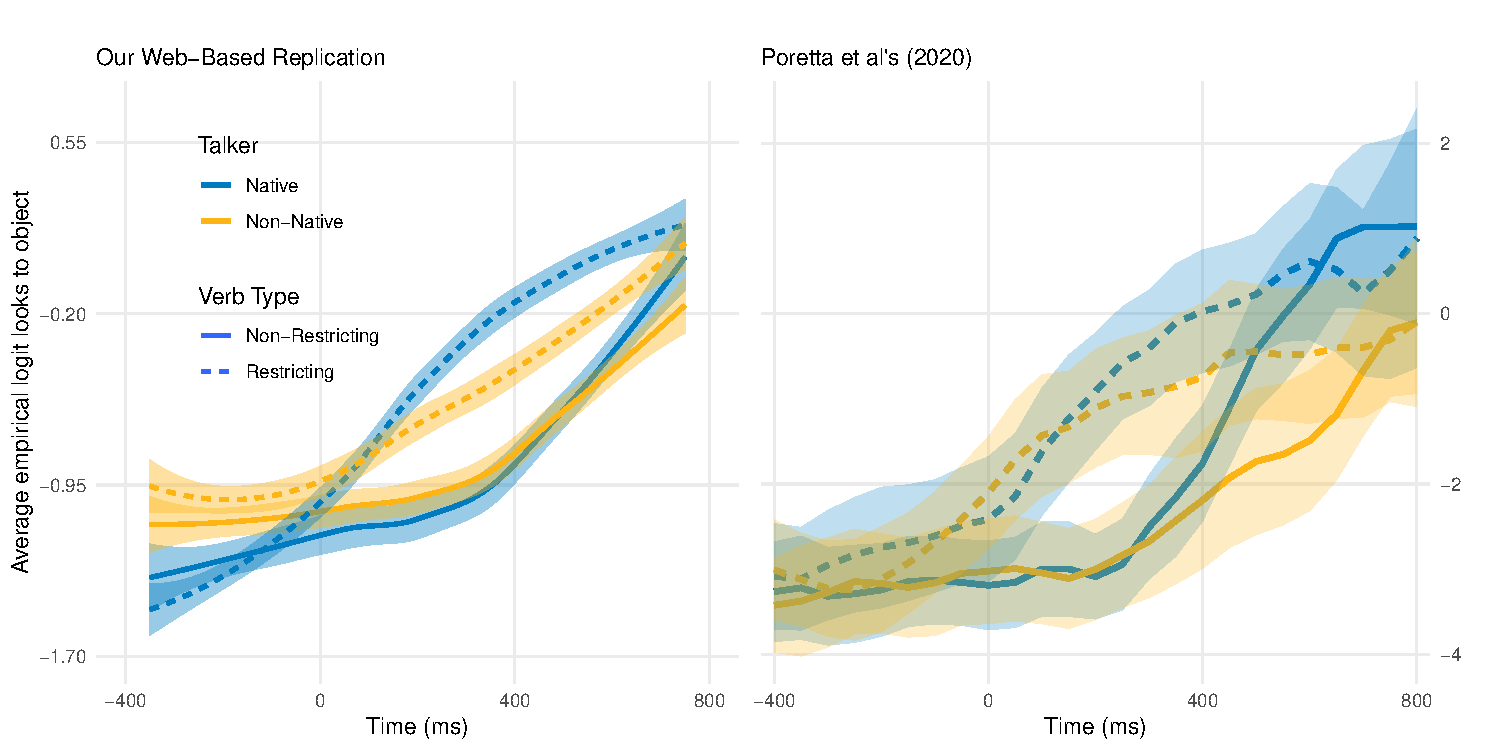
\includegraphics[width=\textwidth]{figures/smooth_comparison_plot.pdf}
    \caption{Left: our Data. right \parencite{Porretta_et_al_2020}}
    \label{fig:smooth}
\end{figure}

Our final data frame in L: 392 was a finishing point. At that point we have two data sets

Good visuals and clean analysis make or break a study. However, these visuals we can implement minor adjustments to create data frames that are optimal for







\lstinputlisting[language=R, firstnumber=last]{scripts/chunk-All Data: Preparing for Models.R}


GAMMS and GLMERS both have there own advantages and disadvantages \parencite{Ito_Knoeferle_2022}

\subsection{Mixed Effects Modeling}
Final model and visualization preparation, 

\lstinputlisting[language=R, firstnumber=last]{scripts/chunk-GLMER: Leveling the Data.R}


%Mixed-effect logistic regression was carried out in R [6], formula: glmer(target ~ talker accent * verb type + (1| item)+(verb type||Participant), family= binomial)). Like [1]’s model, our model yielded an effect of verb type for the restrictive condition (β = 0.08, SE = .04, t = 2.28, p = .029) indicating that prediction occurs irrespective of accent. Additionally, our model found neither an effect of talker accent nor a two-way interaction, thus mirroring the results of [1].

\subsection{Growth Curve Analysis}

Another possible model to use is Growth curve analysis. Prolly not cause space but it seems so logical here. glmer:linear-> GCA:manual polynomials (relax linearity)-> GAMM:automated polynomials (forget about linearity)


\subsection{Generalized Additive Modeling}

\lstinputlisting[language=R, firstnumber=last]{scripts/chunk-GAMM: Leveling the Data.R}

GAMMS are becoming increasingly popular as they allow the research to model complex time course information without the need for assumptions of linearity.

include comparitive visual of 
\begin{figure}[h]
    \centering
    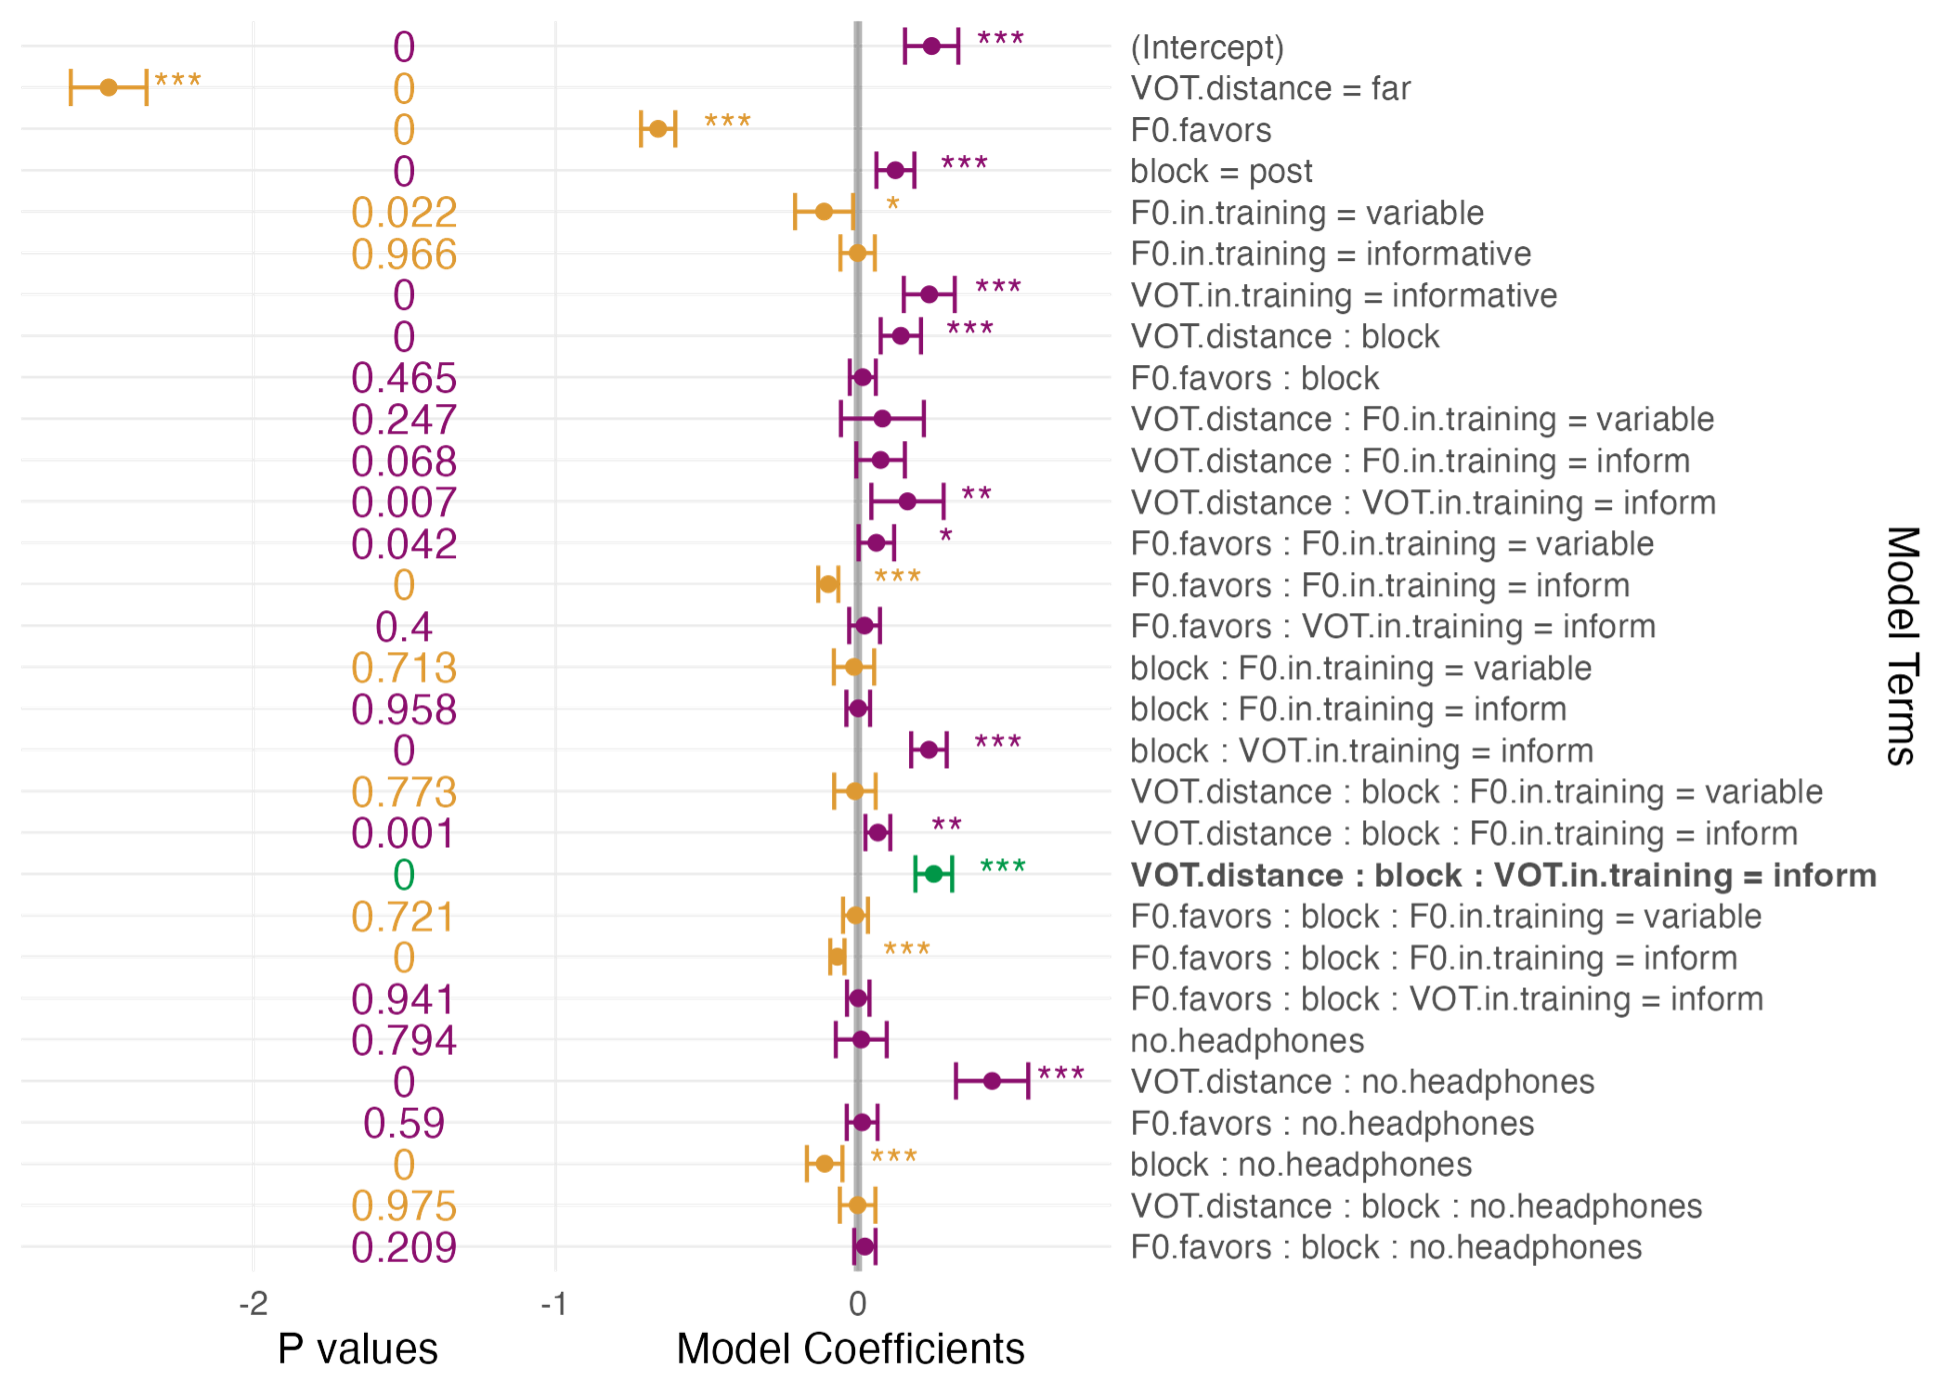
\includegraphics[width=\textwidth]{figures/model_outputs}
    \caption{place holder for real model outputs later}
    \label{fig:model_outputs}
\end{figure}